% Chapter 1

\chapter{Prototype II} % Main chapter title

\label{prototytpe2chapter} % For referencing the chapter elsewhere, use \ref{Chapter1} 

\lhead{Chapter 1. \emph{Prototype II}} % This is for the header on each page - perhaps a shortened title

%----------------------------------------------------------------------------------------
\section{Prototype Development Iteration II}
I started the next iteration of prototype development that aimed to improve the first prototype described in the chapter \ref{prototype1chapter}. In the second prototype the emphasis was more on improving support for the three psychological needs from self-determination theory \citep{ryan2000:self} which are relatedness, competence, and autonomy. I substituted Facebook social plugins with features that could allow users to directly comment on or like each other. Facebook social plugins failed to integrate seamlessly with the app since the network signal was a bit poor in the area where I conducted experiments, therefore users failed to load them into the app. In addition, the system comprised SMS reminders and feedbacks instead of Facebook based reminders. The new system (Figure \ref{figure:prototype_2_screens} ) had the following features of which most of them were improvements from the previous prototype:
\begin{enumerate}
\item{Recording of meals} consumed by a beneficiary user.
\item{A pedometer} for detection of steps walked by beneficiary user.
\item{Pie charts} that show summaries of food groups consumed by a beneficiary user.
\item{Bar charts} that show steps walked by a beneficiary user (daily intervals, 7 days intervals, and, weeks of a month intervals).
\item{Avatars} that can be changed in order to increase autonomy of intermediary users.
\item{Badges} that can be earned through a combination of steps walked by a beneficiary participant and the number of days they app has been utilized by a pair of users. In the previous prototype it was easier to jump from the lowest badge to the highest without passing through intermediate badges as longer as a pair had enough clicks. Therefore, to move to a higher badge in this second prototype a pair was required to use an app for a certain number of days and then couldn't by [ass any badge as the process was incremental. To reach the highest badges pairs were required to pass through all the badges in between in different days, and also to meet requirements for the King/Queen badge which were at least an average of ten thousand (10000) steps walked by a beneficiary user in a day, and at least 18 days of usage activity detected from the app. 
\item{Score board/ leader board} of which points were earned by averaging between points scored from usage (i.e each day of usage resulted into 1000 points earned) and points earned as the result of beneficiary's average number of steps walked (i.e. if the average is \emph{n} steps/day then the number of points accumulated is ``n'')
\item{Botanical gardens} that consisted of trees and flowers. Trees on the garden grows proportional with badges while flowers grows proportionally with number of meals recorded. if a recorded meal contains fruits and vegetables it is an added advantage.
\item{Fish tanks or bowls / Aquarium} that consisted of Fish of different species. Number of species grows proportional with badges while the size of each specie is proportional to number of meals recorded. If a recorded meal contains fruits and vegetables it is an added advantage on the size.
\end{enumerate}

\begin{figure}[htbp]
  \centering
    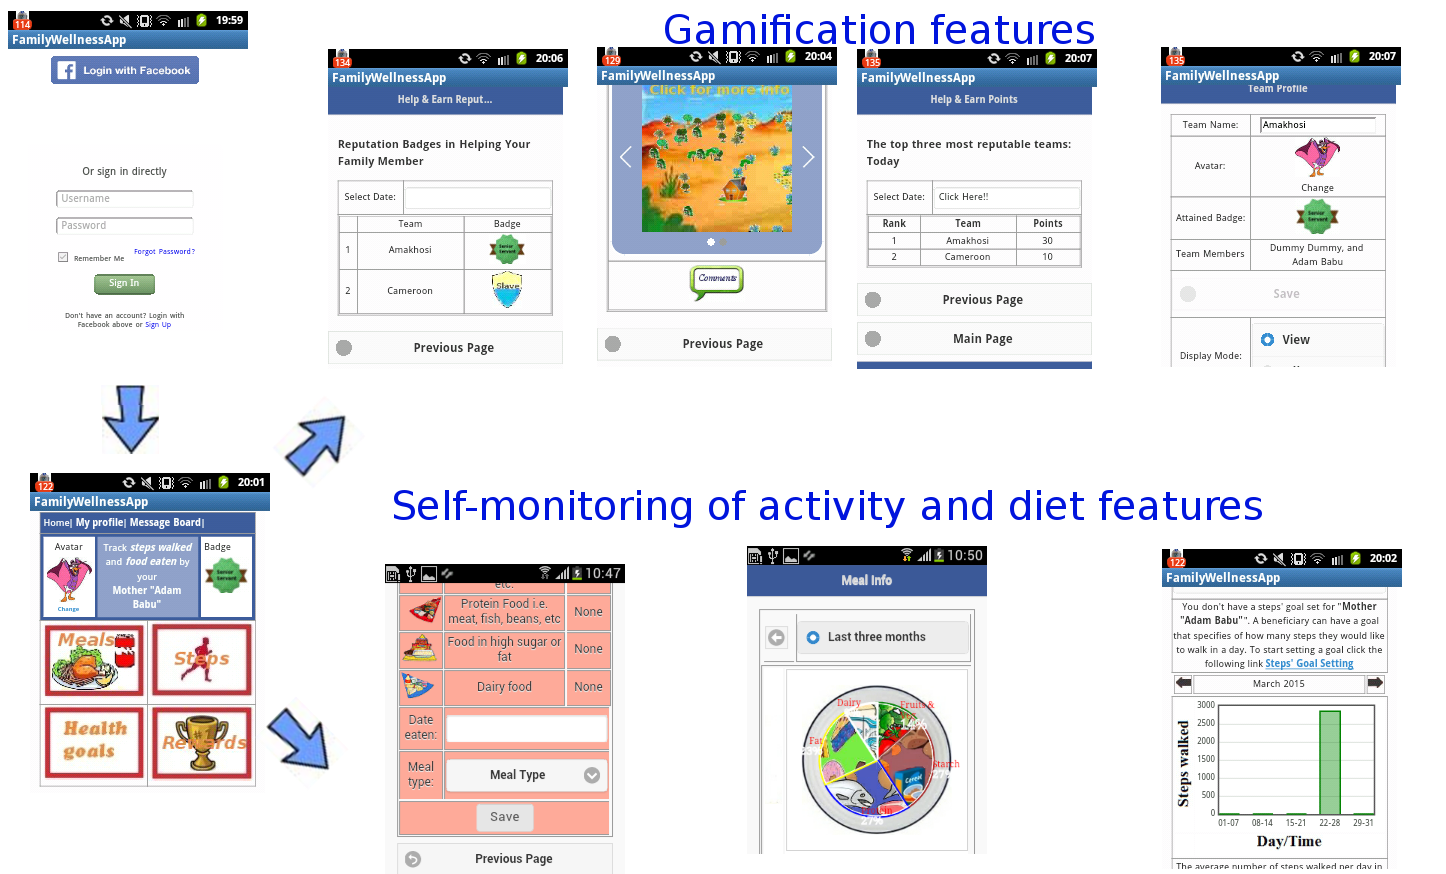
\includegraphics[width=0.8\textwidth]{Figures/Version2/Prototype2Screenshots.png}
    \rule{35em}{0.5pt}
  \caption{Sample screen-shots of the second prototype}
  \label{figure:prototype_2_screens}
\end{figure}

These rules were just arbitrary. The objective was to set challenges in order to increase engagement between intermediaries and beneficiaries when the two users negotiate in interacting with the app.
\section{Prototype Evaluation Description}
The plan in evaluation was to recruit another group of participants. The NGO facilitated access to a group which resided in another side of Philippi where evaluation of the first prototype was conducted. The recruitment was facilitated by the same NGO in Evaluation. But the plan didn't materialize as the NGO advised that we try to look for a different group because the group they were working with expressed concerns regarding safety issues after they heard that they were going to be given phones to use throughout the evaluation period. The NGO was concerned of safety of researchers since rumour had spread throughout the community that someone is going to bring phones to that area. This poses risks to both prospective participants and the researcher. In response to that, this plan was revised and the researcher found another township called Langa, which was a bit smaller and more central township, safer than Philippi.

A research facilitator who is a resident of Langa helped with the recruitment process. This time the recruitment criteria were more stringent compared to the previous evaluation. One of the criteria was to have intermediaries that cohabit or live nearby the beneficiaries. Preference was given to school going children as there were more likely to be interested in gamification. A total of nine adult participants were recruited for the study. The distribution between male and female was three(3) and six(6) respectively. Their average age was 49.3 years old (SD=7.9 years). Each adult participants brought one intermediary participant and formed a pair. The distribution of intermediary participants by gender was 3 males and 6 females. The mean age of these intermediary participants was 14 years old (SD=4.3).  Eight adults  were relatives/familial related to intermediary participants while the remaining adult was just a tenant of her intermediaries' grandmother. Eight intermediary participants were school-going children.

Prior to commencement of the study, both beneficiary and intermediary participants were given information about the study. Participants were informed that the study's cellphone will be collecting their information related to usage of the app, step walked,  and diet and this information will transferred to the researcher's computer at University of Cape Town. All participants who were not minors signed informed consent forms while minors signed assents forms that were also signed by their respective guardians/parents.

Once consent and assent forms were signed, one day was allocated to train intermediary participants on use to use the app. After the training each pair was provided with an one android phone ((Samsung
GT-S5300) that contained two native app. The first app was a pedometer which was not displaying any useful information apart from raw steps' data. The pedometer task was to send these steps to a server so that they can be presented  and viewed in a better format through a web application. The second app provided a link to the web application so that users don't have to type a URL every time they needed to access the web app.

In order to encourage participation, each beneficiary participant received ZAR 40 worth of airtime four times in a period of three weeks (ZAR 160 in total). To encourage participation of intermediary participants, each pair was credited 300MB of data to use on the Android phone as it was expected that intermediaries would borrow phones to access other things on the internet that are beyond prescribed uses.

I left the app in the field for three weeks before conducting an evaluation. After three weeks I conducted the evaluation which is described on the next sub-section.
\section{Prototype Evaluation Methods}
The evaluation relied in two approaches which are collecting user logs and interviews. In interviews, all respondents were familiar/comfortable with English, therefore, interviews were conducted in English. A total of three(3) intermediary participants, and five(5) intermediary participants were interviewed. These are the only participants that I could reach to during the time of interviews. These were short interviews which lasted up to 15 minutes for one person. 
\section{Findings}
The key important findings were based on social factors that influenced usage of the app. Some of the findings from this chapter together with findings from the previous chapter (Chapter \ref{prototype1chapter}) have also appeared in a conference paper that I co-authored \citep{katule2016leveraging}. 
\begin{flushright}
\end{flushright}
